\apendice{Plan de Proyecto Software}

\section{Introducción}
En cualquier proyecto de este tipo es relevante incluir cierta información sobre la planificación, viabilidad y análisis de costes en el desarrollo del mismo con la finalidad de conseguir una visión de cómo ha ido evolucionando el proyecto y los ciclos de trabajo que se han llevado a cabo.

He de señalar que en la última tercera parte de los sprints, no siempre he contado con una línea de datos con la que poder replicar datos en GitHub, por lo que se han generado menos commits de los que se hubiera hecho si hubiera contado con medios a mi alcance. En cualquier caso, se ha intentado maximizar el número de puntos de salvado para que quedase constancia de la evolución del proyecto. Además, al redactar el proyecto en \LaTeX{} desde la plataforma de Overleaf no refleja el tiempo real invertido puesto que no se realizan cambios en el repositorio de forma automática, hasta que compilo, descargo y actualizo el repositorio manualmente.

En el primer apartado trataremos la~\textbf{planificación temporal}, donde podremos ver como han evolucionado los tiempos de trabajo durante las semanas en las que se ha trabajado en el proyecto. En el segundo apartado se reflejará un \textbf{estudio de viabilidad} sobre el proyecto, que a su vez incluye dos partes, la parte económica y la parte legal.

\section{Planificación temporal}
Al comenzar el proyecto se determinó que se utilizaría una metodología ágil para hacer el desarrollo del proyecto pero esta decisión ha terminado siendo un hándicap producido por la falta de documentación y la dudosa credibilidad de muchas páginas web y documentación que he encontrado, y se ha traducido en una gran inversión en tiempo.

Ante todo, se ha intentado seguir un mínimo de pautas~\textbf{Scrum}~\cite{manual:Scrum} pese a no existir un grupo de trabajo real con unas tareas diarias y roles definidos:
\begin{itemize}
    \item Las tareas fueron siempre semanales en forma de <<sprints>>.
    \item Al finalizar el sprint se hace la entrega del trabajo elaborado en la semana y se determinan las próximas tareas.
    \item Tras determinar las tareas se definen los <<milestones>> y los <<issues>>.
    \item Para hacer el seguimiento de las tareas se ha utilizado en tablero~\textbf{Kanban} de~\textbf{ZenHub}.
    \item Tras finalizar el sprint se puede comprobar el trabajo mediante los~\textit{gráficos burndown}.
\end{itemize}

Las reuniones de trabajo han sido consensuadas y planificadas para realizarlas los jueves de cada semana, con el siguiente resultado:

\subsection{Sprint 00 - 01/10/2020 - 08/10/2020}
En la primera reunión nos reunimos Álvar Arnaiz González y yo. En ella hice la propuesta de temática del TFG y, además expuse diferentes ideas y enfoques sobre el proyecto en la que se determinó a grandes rasgos la posible viabilidad del proyecto.
Los objetivos de este <<sprint>> introductorio fueron la búsqueda de repositorios y otros proyectos para tomar ideas o si era posible hacer algún fork. También, el estudio la estructura del proyecto y herramientas software e interfaces a utilizar.

\subsection{Sprint 01 - 09/10/2020 - 15/10/2020}
Tras determinar el enfoque final de proyecto, se consensuó que los objetivos de este sprint fueron la búsqueda de información relevante, otros proyectos y recursos que pudieran servir de utilidad como pueden ser APIS. Se buscaron algunas páginas web para realizar pruebas de extracción de datos con <<web scraping>>~\footnote{Se trata brevemente en el punto 4 de la memoria} y se descompusieron las tareas en unidades pequeñas de trabajo para poder afrontarlas durante sprints.

En este sprint también generé el repositorio en GitHub para poder trabajar contra él y podemos ver las líneas de código utilizadas en el \href{https://github.com/davidelinformatico/TFG/issues/1}{primer \textit{issue}}.

\subsection{Sprint 02 - 16/10/2020 - 22/10/2020}
Los objetivos de este sprint fueron el buscar repositorios, APIS, servicios y tecnologías con las que darle forma al proyecto. Se decidió generar algún tipo de aplicación desde la que poder controlar la instalación haciéndola más amigable y con mejor capacidad de interacción. Se investigan opciones.

En el~\href{https://github.com/davidelinformatico/TFG/issues/2}{issue 2} se hizo una búsqueda por la web para buscar repositorios y proyectos sobre domótica.

En el~\href{https://github.com/davidelinformatico/TFG/issues/3}{issue 3} buscamos algunas APIS para orientar el proyecto hacia el uso de APIS destinadas a ofrecer información que pueda servirnos y se realizaron algunas pruebas.

En el~\href{https://github.com/davidelinformatico/TFG/issues/4}{issue 4} se realizó un pequeño estudio de las tecnologías que podríamos utilizar, desde el procesador de textos, que finalmente se utilizó~\LaTeX{}, como la revisión de las normativas electrotécnicas que debía seguir en el proyecto y también se determinó la utilización de Telegram para interactuar con el Sistema Domótico.

\subsection{Sprint 03 - 23/10/2020 - 29/10/2020}
Los objetivos de este sprint fueron determinar los componentes hardware necesarios para completar el proyecto y se realiza la compra de material.
En todos los <<issues>> del <<\href{https://github.com/davidelinformatico/TFG/milestone/3?closed=1}{milestone 3}>> podemos ver múltiples enlaces, comparativas, justificaciones e imágenes en las que se ha basado toda la instalación física posterior.

\subsection{Sprint 04 - 30/10/2020 - 05/10/2020}
Se incorpora D.Alejandro Merino Gómez al que se le presenta el proyecto y se le concede acceso a los repositorios para que pueda co-tutorizar el proyecto.

Los objetivos de este <<milestone>> fueron todos de la parte física de la instalación:
Podemos ver en el \href{https://github.com/davidelinformatico/TFG/issues/15}{issue 15} que finalicé la tirada de cable junto a un diagrama explicativo del funcionamiento de un pulsador de 3 posiciones (Posición 1, Reposo y Posición 2. Teniendo en cuenta que las dos posiciones que dan continuidad al circuito tienen invertida la polaridad).

También vemos en el \href{https://github.com/davidelinformatico/TFG/issues/16}{issue 16} la presentación de la Raspberry Pi que utilizaremos, los conectores del tipo JST-XH que se han utilizado en el crimpado de los cables electrónicos, los cables finalizados con sus conectores y la disposición final de la Raspberry Pi en su ubicación final de la instalación.

\subsection{Sprint 05 - 06/11/2020 - 12/11/2020}
Se repasan los cambios propuestos y se incluyen otros nuevos sobre la parte física de la instalación. Se hace el seguimiento de la instalación y se comentan las fotos y el estado de la instalación.
Los objetivos de este sprint son todos aquellos que sean necesarios para la adecuación del software básico para comenzar el proyecto como la actualización del sistema operativo o instalación de software adicional. Además se deben valorar opciones para controlar los GPIO.

Vemos en los issues \href{https://github.com/davidelinformatico/TFG/issues/21}{21} y \href{https://github.com/davidelinformatico/TFG/issues/19}{19} las configuraciones básicas realizadas a nuestro Raspbian. Para explicar este proceso grabé dos vídeos, titulados \href{https://youtu.be/B8E6q1fLp7Q}{Primeros Pasos Raspberry Pi} y \href{https://youtu.be/Vz38sGYpcYQ}{Actualización de Raspberry Pi y configuración básica}, respectivamente.

\subsection{Sprint 06 - 13/11/2020 - 19/11/2020}
Se revisan los puntos anteriores y se compone un tablero de pruebas de forma que se puede controlar el encendido de una bombilla desde nuestra Raspberry Pi. También se graba un vídeo explicativo y se diseñan unos diagramas explicativos.

Podemos ver en el \href{https://github.com/davidelinformatico/TFG/issues/22}{issue 22} que se presenta un diagrama con la lista de los componentes que vamos a utilizar en el tablero de pruebas y un diagrama de como se compondrá el tablero. En este issue también grabé un vídeo para explicar el tablero de pruebas y decidí utilizar un efecto visual más conservador de cara al final del proyecto.

En el \href{https://github.com/davidelinformatico/TFG/issues/23}{issue 23} he explicado cómo se controlan los GPIO de nuestra Raspberry Pi desde su distribución Linux~\footnote{Raspbery pi (Raspbian OS).} desde Bash y desde Python.

\subsection{Sprint 07 - 20/11/2020 - 26/11/2020}
Se realiza una investigación sobre como se puede implantar el bot en nuestro proyecto, se realiza el primer código de pruebas y se presentan las primeras pruebas con el bot. Podemos ver en el \href{https://github.com/davidelinformatico/TFG/issues/13}{issue 13} un resumen de las pruebas que estuve realizando con los diferentes teclados de que dispone Telegram.
También, se proponen correcciones en la redacción.

\subsection{Sprint 08 - 27/11/2020 - 03/12/2020}
En el \href{https://github.com/davidelinformatico/TFG/milestone/8?closed=1}{milestone 8}, podemos ver que se incluyen varios issues.

El código se divide en tres partes, la parte automática, la parte de control mecánico y la parte del bot. 

En este issue se genera la primera ejecución de forma autónoma de la parte automática del proyecto utilizando CRON y lo pasamos del entorno de pruebas a un entorno de producción en fase experimental. En este momento únicamente tenemos control sobre la máquina de forma física o por VNC.
Por último, se presentan las primeras funcionalidades del bot, se proponen cambios y mejoras.

\subsection{Sprint 09 - 04/12/2020 - 10/12/2020}
En el \href{https://github.com/davidelinformatico/TFG/milestone/9?closed=1}{milestone 9} se revisan las funcionalidades del Bot~\cite{misc:TelegramApi} de Telegram~\cite{misc:TelegramApp} que utilizaremos, se proponen cambios y mejoras en el código preexistente en fase de pruebas.

Finalmente se integra un bot de Telegram completamente funcional desde el que podremos lanzar órdenes a nuestro sistema domótico con los scripts existentes.

\subsection{Sprint 10 - 11/12/2020 - 17/12/2020}
En el \href{https://github.com/davidelinformatico/TFG/milestone/10?closed=1}{milestone 10} se ha aprovechado para optimizar las rutas de los archivos a los que se invoca desde el código en ejecución y se han modificado algunas salidas para que tengan un aspecto visual más atractivo, incluyendo tablas y emoticonos desde Unicode~\cite{misc:UnicodeWikipedia}.

Se comprueban las funcionalidades proponiendo cambios funcionales y de estilos de forma que se pueda interactuar contra el bot y se muestren los mensajes en un formato más atractivo. También se propone unificar las rutas de trabajo de los diferentes scripts.



\subsection{Sprint 11 - 18/12/2020 - 24/12/2020}
Se propone estructurar el código por funcionalidades (obtención de información de la web, y por otro lado, modificación de archivos del sistema) y se proponen cambios en la redacción a implementar en el sprint 12.


Finalmente, se ha conseguido generar la división del código en 3 archivos principales:

De esta manera conseguimos minimizar las comunicaciones con el exterior y poder ejecutar cada unidad de código de forma aislada en caso de necesitarlo puesto que se ha estructurado por funcionalidad. Un ejemplo puede ser cuando se modifica la hora de subida de las persianas, el módulo de generación de CRON leería el archivo de parámetros personalizados y generaría la configuración a partir de éstos.


\subsection{Sprint 12 - 25/12/2020 - 31/01/2021}
Se finaliza la redacción de la memoria, antes de la revisión final del texto, y se comienza con los anexos. Además se realiza un depurado manual del código y también se utiliza SonarCloud~\cite{misc:sonarcloud}.

\subsection{Sprint 13 - 01/12/2020 - 07/01/2021}
Redacción de los anexos, corrección de la memoria y limpieza de código.
Se ha proporcionado la primera Release estable~\texttt{v1.0} y asignado la licencia del proyecto.

\subsection{Sprint 14 - 08/01/2020 - 14/01/2020}
Corrección de los anexos y se sube la Release~\texttt{v1.1} con mejoras en el código: se incluyen los archivos generadores de archivos de control y mejoras en los archivos de instalación.

\subsection{Sprint 15 - 15/01/2020 - 20/01/2020}
Se sube la versión~\texttt{v1.2} en la que se eliminan archivos duplicados en el código, se limpia de incorrecciones y se comentan las funciones y scripts. También se sube la versión~\texttt{v1.3}, final. En la que se mejoran algunas salidas de datos.
Se realizan las grabaciones y edición de los vídeos, así como la entrega del proyecto.


\section{Estudio de viabilidad}
El estudio de viabilidad es inherente a cualquier proyecto y determina si éste puede ser aplicable o no, y también sirve para aclarar algunos puntos importantes para ayudar a la toma de decisiones ejecutivas:
\begin{itemize}
    \item Señalar las características únicas propias del proyecto en cuestión que permitan poder realizar un estudio de riesgos.
    \item Enmarcar legalmente el proyecto a realizar y determinar el nicho de mercado en que encaja.
    \item Poder ajustar el presupuesto del proyecto a las necesidades existentes.
\end{itemize}

\subsection{Viabilidad económica}
En este punto que se tratarán los detalles económicos del proyecto, que son una parte fundamental para saber si el proyecto se puede asumir en un proyecto con carácter comercial desde el ámbito empresarial con carácter profesional.

En esta sección se explica cada uno de los costes asociados al proyecto teniendo en cuenta que se ha intentado minimizar los costes en todos y cada uno de los puntos de la instalación y material.

\subsubsection{Coste de personal}
Aún habiendo sido desarrollado por una única persona, el apartado de costes de personal es el que contiene un gasto mayor con respecto al resto de apartados económicos.

Se ha estimado un sueldo de 22.000€ brutos anuales en 12 pagas, para realizar el cálculo en el intervalo entre el 01 de octubre de 2020 y el 20 de enero de 2021. Si hacemos el cálculo de estos 111 días que ha durado el proyecto, vemos que se corresponde a 3,7 meses de trabajo por lo que el gasto total en personal durante el proyecto asciende a 8.818,33€.
El desglose mensual podemos verlo en la tabla~\ref{tab:CostePersonal} y el coste total en la tabla~\ref{tab:CostePersonalTotal}.~\\~\\~\\~\\ % para evitar que corte la tabla, que dificulta la lectura.

\begin{longtable}[c]{@{}lrr@{}}
\toprule
\multicolumn{1}{c}{\textbf{Concepto}} & \multicolumn{1}{c}{\textbf{Porcentaje}} & \multicolumn{1}{c}{\textbf{Coste}} \\* \midrule
\endfirsthead
%
\endhead
%
\bottomrule
\endfoot
%
\endlastfoot
%
Sueldo Base (Neto) &  & 1833,33 € \\
Contingencias Comunes & 23,60 \% & 432,67 € \\
Tipo general & 5,50 \% & 100,83 € \\
Fogasa & 0,20 \% & 3,67 € \\
FP & 0,70 \% & 12,83 € \\ \hline
\textbf{Total Gasto Mensual (Suma)} & & \textbf{2.383,33 €} \\* \bottomrule \\
\caption{Coste de personal mensual}
\label{tab:CostePersonal}
\end{longtable}


\begin{longtable}[c]{@{}ll@{}}
\toprule
\centering
\multicolumn{1}{c}{\textbf{Concepto}} & \multicolumn{1}{c}{\textbf{Coste}} \\* \midrule
\endfirsthead
%
\endhead
%
\bottomrule
\endfoot
%
\endlastfoot
%
Número de meses & 3.7 meses \\
Gasto mensual & 2.383,33 € \\ \hline
\textbf{Total Gasto Proyecto} & \textbf{8.818,33 €} \\* \bottomrule \\
\caption{Coste total en personal durante el proyecto}
\label{tab:CostePersonalTotal}\\
\end{longtable}


Para realizar el cálculo me he apoyado en la documentación oficial que tiene a disposición del ciudadano la Seguridad Social en su página web~\cite{manual:SS}. En ella podemos ver que hay que aportar un 23,60~\% en concepto de Contingencias comunes, un 5,50~\% en concepto de desempleo de Tipo general, un 0,20~\% a FOGASA y un 0,70~\% para FP.



\subsubsection{Coste hardware}
Aunque se ha procurado ahorrar en costes de hardware, y sabiendo que este proyecto se puede realizar íntegramente desde la misma máquina Raspberry Pi que se ha utilizado para desarrollar y que puede se trabajar conectado a la máquina, incluiré un equipo portátil de gama corporativa desde el que trabajar cómodamente.

Tras valorar las características de las diferentes Raspberry Pi, y sabiendo la potencia que necesita el proyecto, adquiriría la versión 3B+ por disponer de mayor potencia y mejor conectividad por una inversión razonable aunque para el proyecto 'reciclaré' una RbP 2B que tengo en desuso. Por ello, en el apartado económico figurará la versión 3B a un precio de 34,30€. El estudio preliminar se realizó en el milestone 3~\cite{misc:Milestone3} y puede observarse online mientras que el coste final se representa en la tabla~\ref{tab:CosteHW}

Para calcular la amortización del material en el tiempo transcurrido he determinado un periodo de amortización de 5 años, de los cuales han transcurrido 3,7 meses.

\begin{longtable}[c]{@{}lrr@{}}
\toprule
\centering
\multicolumn{1}{c}{\textbf{Concepto}} & \multicolumn{1}{c}{\textbf{Coste}} & \multicolumn{1}{c}{\textbf{Coste amortizado}} \\* \midrule
\endfirsthead
%
\endhead
%
\bottomrule
\endfoot
%
\endlastfoot
%
Portátil Lenovo Thinkpad T50 & 1.427,86 € & 88,05 € \\
Raspberry Pi 2B & 34,30 € & 34,30 € \\
Tarjeta SD & 14,08 € & 14,08 € \\
Cable UTP5e & 14,41 € & 14,41 € \\
Caja Raspberry Pi & 15,28 € & 15,28 € \\
Placa Board & 3,50 € & 3,50 € \\
Dongle WiFi & 6,95 € & 6,95 € \\
Relés & 38,35 € & 38,35 € \\
Cables electrónica & 6,59 € & 6,59 € \\
Conectores de cables electrónicos & 10,70 € & 10,70 € \\
Crimpadora JST & 12,00 € & 0,74 € \\
Guía pasacables & 2.50 € & 0.15 € \\ 
\textbf{Total} & \textbf{1.586,52 €} & \textbf{233,11 €} \\ \bottomrule \\
\caption{Coste total en hardware}
\label{tab:CosteHW}
\end{longtable}

\subsubsection{Coste software}
Como el único programa que debemos correr en una máquina local, lo podemos hacer sobre Linux, utilizaremos este Sistema Operativo para ahorrar en costes. El único gasto es la licencia del programa Fritzing, que tiene un costo total de 8€~\cite{misc:Fritzing}.

\subsubsection{Costes varios}
Únicamente incluiré una tarifa de datos y una de móvil por un precio de 50€/mes.
El motivo es que se necesita un número de teléfono móvil para poder hacer pruebas con Telegram aunque lo ideal es utilizar dos números de teléfono para hacer algunas pruebas.
Además, debemos incluir gastos generales de oficina. El cálculo se ha realizado sobre el último precio publicado de un vivero de empresas de Getafe. El precio asciende a 7,48€/$m^{2}$ al mes IVA.exc, por lo que mensualmente pagaremos 108,60€ por una oficina de 12$m^{2}$.

En total, en este subpunto, tenemos un coste mensual de 158,60€. Al tener que mantenerlo 4 meses, el precio asciende a 634.40€.

Podemos comprobar el precio público en~\url{https://www.getafeiniciativas.es/empresas/espacios-para-empresas/centro-municipal-de-empresas/vivero-de-empresas}.

\subsubsection{Coste Total}
Si sumamos los costes anteriormente descritos, vemos que la suma asciende a \textbf{9693,84 €} que han quedado descritos en la tabla~\ref{tab:CosteTotal}.

\begin{longtable}[c]{@{}lr@{}}
\toprule
\centering
\multicolumn{1}{c}{\textbf{Concepto}} & \multicolumn{1}{c}{\textbf{Coste}} \\* \midrule
\endfirsthead
%
\endhead
%
\bottomrule
\endfoot
%
\endlastfoot
%
Personal & 8.818,33 € \\
Hardware & 233,11 € \\
Software & 8 € \\
Costes varios & 634,40 € \\\midrule
\textbf{Total} & \textbf{9693,84 €} \\ \bottomrule \\
\caption{Tabla de costes totales} 
\label{tab:CosteTotal}
\end{longtable}

\subsection{Beneficios}
En un principio el proyecto está pensado para ser utilizado de forma libre pero, en el caso de cambiar de idea se puede monetizar de varias formas. Quizás, la más sencilla sea un pago por licencia con carácter anual pudiendo poner una suscripción de 1€ o 2€ por cada mes de uso en cada instalación de forma que se podría rentabilizar rápidamente como se ha plasmado en la tabla~\ref{tab:Cuotas1}.


\begin{longtable}[c]{@{}lrrr@{}}
\toprule
\centering
\multicolumn{1}{c}{\textbf{Tiempo}} & \multicolumn{1}{c}{\textbf{1 Instalación}} & \multicolumn{1}{c}{\textbf{2 Instalaciones}} & \multicolumn{1}{c}{\textbf{3 Instalaciones}}\\* \midrule
\endfirsthead
%
\endhead
%
\bottomrule
\endfoot
%
\endlastfoot
%
1 año & 12€ & 24€ & 36€ \\
2 años & 22€ & 45€ & 50€ \\ \bottomrule \\
\caption{Cuotas para la posible monetización}
\label{tab:Cuotas1}
\end{longtable}

\subsection{Viabilidad legal}
Tanto en el proyecto como en los anexos se ha hecho alusión a algunas licencias como <<Creative Commons~\cite{wiki:Creative}>> y <<GNU~\cite{manual:GNU}>>. En este apartado se detalla el marco legal del proyecto, pero para poder entenderlo debemos entender que es una licencia:

\begin{displayquote}
\Chapter{\textit{Una licencia de software es un contrato entre el licenciante (autor/titular de los derechos de explotación/distribución) y el licenciatario (usuario consumidor, profesional o empresa) del programa informático, para utilizarlo cumpliendo una serie de términos y condiciones establecidas dentro de sus cláusulas, es decir, es un conjunto de permisos que un desarrollador le puede otorgar a un usuario en los que tiene la posibilidad de distribuir, usar o modificar el producto bajo una licencia determinada.}}~\cite{misc:WikiLicencia}
\end{displayquote}

Para poder determinar la licencia más adecuada para nuestro proyecto debemos hacer un estudio de las licencias que se utilizan en todo el proceso ya que hemos utilizado licencias a tener en cuenta.

\subsubsection{Frontend}
En el proyecto se ha utilizado un bot de Telegram como FrontEnd del sistema domótico. Podemos ver las licencias del sistema que utilizamos en la tabla~\ref{tab:FrontEnd}.

\begin{longtable}[c]{@{}lll@{}}
\toprule
\centering
\multicolumn{1}{c}{\textbf{Nombre}} & \multicolumn{1}{c}{\textbf{Licencia}} & \multicolumn{1}{c}{\textbf{Descripción}} \\ \midrule
\endfirsthead
%
\endhead
%
\bottomrule
\endfoot
%
\endlastfoot
%
Telegram Code & MIT & Código interno de Telegram \\
Telegram App~\cite{misc:TelegramApp} & GPLv2 y post & Aplicaciones móviles \\
Telegram Api~\cite{misc:TelegramApi} & GPLv3 excepto OpenSSL & API pública de Telegram \\ \bottomrule \\
\caption{Dependencias en el FrontEnd.}
\label{tab:FrontEnd}
\end{longtable}

\subsubsection{Backend}
En la parte de BackEnd nos hemos servido de otros códigos o <<dependencias>> que también cuentan con sus propias licencias, como podemos ver en la tabla~\ref{tab:BackEnd}. Al realizar un pequeño estudio podemos determinar compatibilidad de las licencias de las dependencias utilizadas en nuestro proyecto y que podemos ver en la imagen~\ref{LicenseComp}.~\\~\\ % Se incluye para evitar cortar la tabla y que se lea mejor

\footnotesize%%%%%%%%%%%  smaller font size %%%%%%%%
\begin{longtable}[c]{@{}lccl@{}}
\toprule
\multicolumn{1}{c}{\textbf{Nombre}} & \textbf{Versión} & \textbf{Licencia} & \multicolumn{1}{c}{\textbf{Descripción}} \\ \midrule
\endfirsthead
%
\endhead
%
\bottomrule
\endfoot
%
\endlastfoot
%
Raspbian & 5.4 & GPL & Sistema Operativo de Raspberry Pi \\
Python~\cite{misc:Python} & 3.7 & PSF & Lenguaje de programación interpretado \\
urllib3 & 1.24.1 & MIT & Cliente HTTP \\
datetime & - & ZPL & Módulo para trabajar con fechas y horas \\
pandas & 1.1.4 & BSD & \begin{tabular}[c]{@{}l@{}}Herramienta de manipulación de datos \\ de alto nivel\end{tabular} \\
matplotlib & 3.3.3 & PSF based & Biblioteca   para la generación de gráficos \\
python-telegram-bot & 13.1 & LGPL3 & \begin{tabular}[c]{@{}l@{}}Biblioteca que gestiona \\ la interacción con la API\end{tabular} \\
pyTelegramBotAPI & 3.7.5 & GPL2 & \begin{tabular}[c]{@{}l@{}}Biblioteca que gestiona \\ el funcionamiento del bot\end{tabular} \\
simplejson & 3.16.0 & GPL & Paquete para trabajar con objetos json~\cite{misc:Json} \\
requests & 2.21.0 & Apache 2.0 & Biblioteca HTTP \\
pycurl & 7.43.0.6 & LGPL/MIT & Cliente   HTTP \\
%telegram & 0.0.1 & GPL2 to LGPL3 & Cliente para Telegram \\ 
\bottomrule~\\
\caption{Dependecncias en el BackEnd.}
\label{tab:BackEnd}
\end{longtable}
\normalsize

Tras ordenar las compatibilidades de las licencias de las dependencias de nuestro proyecto vemos que la licencia más compatible es GPL3~\cite{lic:GPL3}, y para evitar interferir de algún modo con las licencias de alguna de ellas, nuestro software cuenta con dicha licencia GPL3.
\begin{figure}[h!]
    \centering
    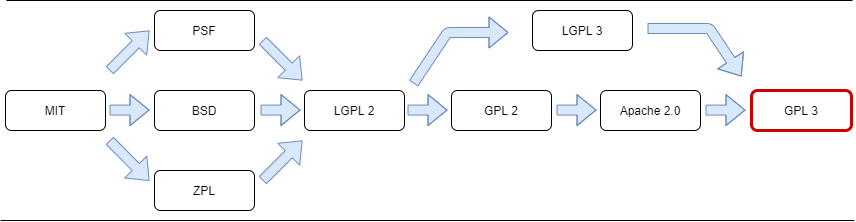
\includegraphics[width=\textwidth]{img/Diagramas/LicenseComp.png}
    \caption{Compatibilidad entre licencias. } \label{LicenseComp}
\end{figure}

El liberar el código bajo GPL3~\cite{lic:GPL3} resulta beneficioso ya que al ser de libre disposición cualquiera puede beneficiarse de éste, del mismo modo que puede mejorarlo y licenciarlo con una licencia libre compatible y poder aprovechar también dichas mejoras en futuros desarrollos. 

Por ello, para entender que permite la licencia GPL3~\cite{lic:GPL3} he confeccionado un breve resumen. Aunque la tabla~\ref{tab:GPL3} no representa la casuística completa de la licencia si nos permite tener una idea global del funcionamiento de ésta.

\footnotesize%%%%%%%%%%%  smaller font size %%%%%%%%
\begin{longtable}[c]{@{}lll@{}}
\toprule
\multicolumn{1}{c}{\textbf{Permitido}} & \multicolumn{1}{c}{\textbf{Limitaciones}} & \multicolumn{1}{c}{\textbf{Obligaciones}} \\* \midrule
\endfirsthead
%
\endhead
%
\bottomrule
\endfoot
%
\endlastfoot
%
Uso Comercial y privado. & \begin{tabular}[c]{@{}l@{}}Se prohíbe la concesión\\de sublicencias.\end{tabular} & Se debe incluir el software original. \\
El código se puede modificar. & Responsabilidad limitada. & \begin{tabular}[c]{@{}l@{}}Debe incluir los cambios en\\ el software.\end{tabular} \\
El código se puede distribuir. & No dispone de garantía. & \begin{tabular}[c]{@{}l@{}}El código debe divulgarse bajo\\una licencia compatible\\con GPL 3.0.\end{tabular} \\
\begin{tabular}[c]{@{}c@{}}Se puede otorgar garantía al \\ código con licencia.\end{tabular} &  & Debe incluir la licencia. \\* \bottomrule 
\caption{GPL3}
\label{tab:GPL3}
\end{longtable}
\normalsize Podemos ampliar la información en la página oficial de GNU~\cite{lic:GPL3}.

\subsubsection{Documentación}

Para generar la documentación se han utilizado dos licencias, la referente a~\LaTeX{} y a la aplicación Fritzing. Los diagramas electrónicos del proyecto han sigo generados con esta licencia Creative Commons by-sa~\cite{lic:CCbysa3}. La documentación del proyecto tiene la misma cobertura CC by-sa, que permite el uso comercial y distribución tanto de esta obra como derivadas de ésta siempre que se cuente con la misma licencia que regula la obra original. Podemos ver los derechos adquiridos de la obra así como las obligaciones en la página oficial~\cite{lic:CCbysa3}.

\begin{longtable}[c]{@{}lll@{}}
\toprule
\multicolumn{1}{c}{\textbf{Nombre}} & \multicolumn{1}{c}{\textbf{Licencia}} & \multicolumn{1}{c}{\textbf{Descripción}} \\* \midrule
\endfirsthead
%
\endhead
%
\bottomrule
\endfoot
%
\endlastfoot
%
\LaTeX{}~\cite{wiki:latex} & LPPL & Procesador de textos \\
Fritzing & CC by-sa & Diagramas electrónicos \\* \bottomrule \\
\caption{Dependecncias en la documentación.}
\label{tab:my-table}\\
\end{longtable}


\subsubsection{Resumen del licenciamiento del presente proyecto}
Para facilitar la búsqueda y comprensión de las licencias con que cuenta el proyecto he generado la tabla resúmen~\ref{tab:licproy} y también pueden ver las licencias en los enlaces correspondientes de GPL3~\cite{lic:GPL3} y CC-BY-SA-3.0~\cite{lic:CCbysa3}.~\\~\\ % Se incluye para evitar que corte la tabla

\begin{longtable}[c]{@{}ll@{}}
\toprule
\multicolumn{1}{c}{\textbf{Recurso}} & \multicolumn{1}{c}{\textbf{Licencia}} \\* \midrule
\endfirsthead
%
\endhead
%
\bottomrule
\endfoot
%
\endlastfoot
%
Código Fuente & GPL3 \\
Documentación & CC-BY-SA-3.0 \\
Imágenes & CC-BY-SA-3.0 \\
Vídeos & CC-BY-SA-3.0 \\* \bottomrule \\
\caption{Licencias que protegen el proyecto.}
\label{tab:licproy}\\
\end{longtable}


\begin{figure}[h]
  \begin{subfigure}
    
\includegraphics[width=0.3\textwidth]{img/Diagramas/gplv3-with-text-136x68.png}
  \end{subfigure}
  \hfill
  \begin{subfigure}
    
\includegraphics[width=0.3\textwidth]{img/Diagramas/ccbysa.png}
  \end{subfigure}
\end{figure}

